% -*- mode Latex; -*-
%
% $Id$
%


\documentclass[a4paper]{report}
\usepackage{amsmath}
\usepackage{graphicx}
\begin{document}
\title{Manual for the use of Regress Pro Ellipsometry}
\author{F. Abbate}
\maketitle
\chapter{Introduction}
Regress Pro is a software to perform analysis of spectropic
ellipsometers of reflectometers. In this manual we will suppose that
you are familiar with the basic concepts of ellipsometry.

With Regress Pro you can define a model to describe the film stack and
you can also model each film layer to descibe its optical
properties. You will be also able to define a fit strategy well suited
to the problem under analysis.

With Regress Pro you will be able to determine the optical properties
of unknown materials or, if you already know the materials, you can
run simple fits to determine the thicknesses of the involved layers.

To characterize the optical properties of the materials Regress Pro
offers different optical models
\begin{itemize}
  \item Cauchy model
  \item Harmonic Oscillators model
  \item Lookup model
\end{itemize}
We will mention also that the EMA models are still not supported by
Regress Pro. The support for these models will be added, if possible,
in one of the next release of the software.

\chapter{Script Definition}
The first step to start to use Regress Pro is to define a film
stack. This can be done by describing the film stack in the ``Script''
tab. The best thing you can do is to start with one of the example
script provided with Regress Pro.
\begin{figure}[!thp]
  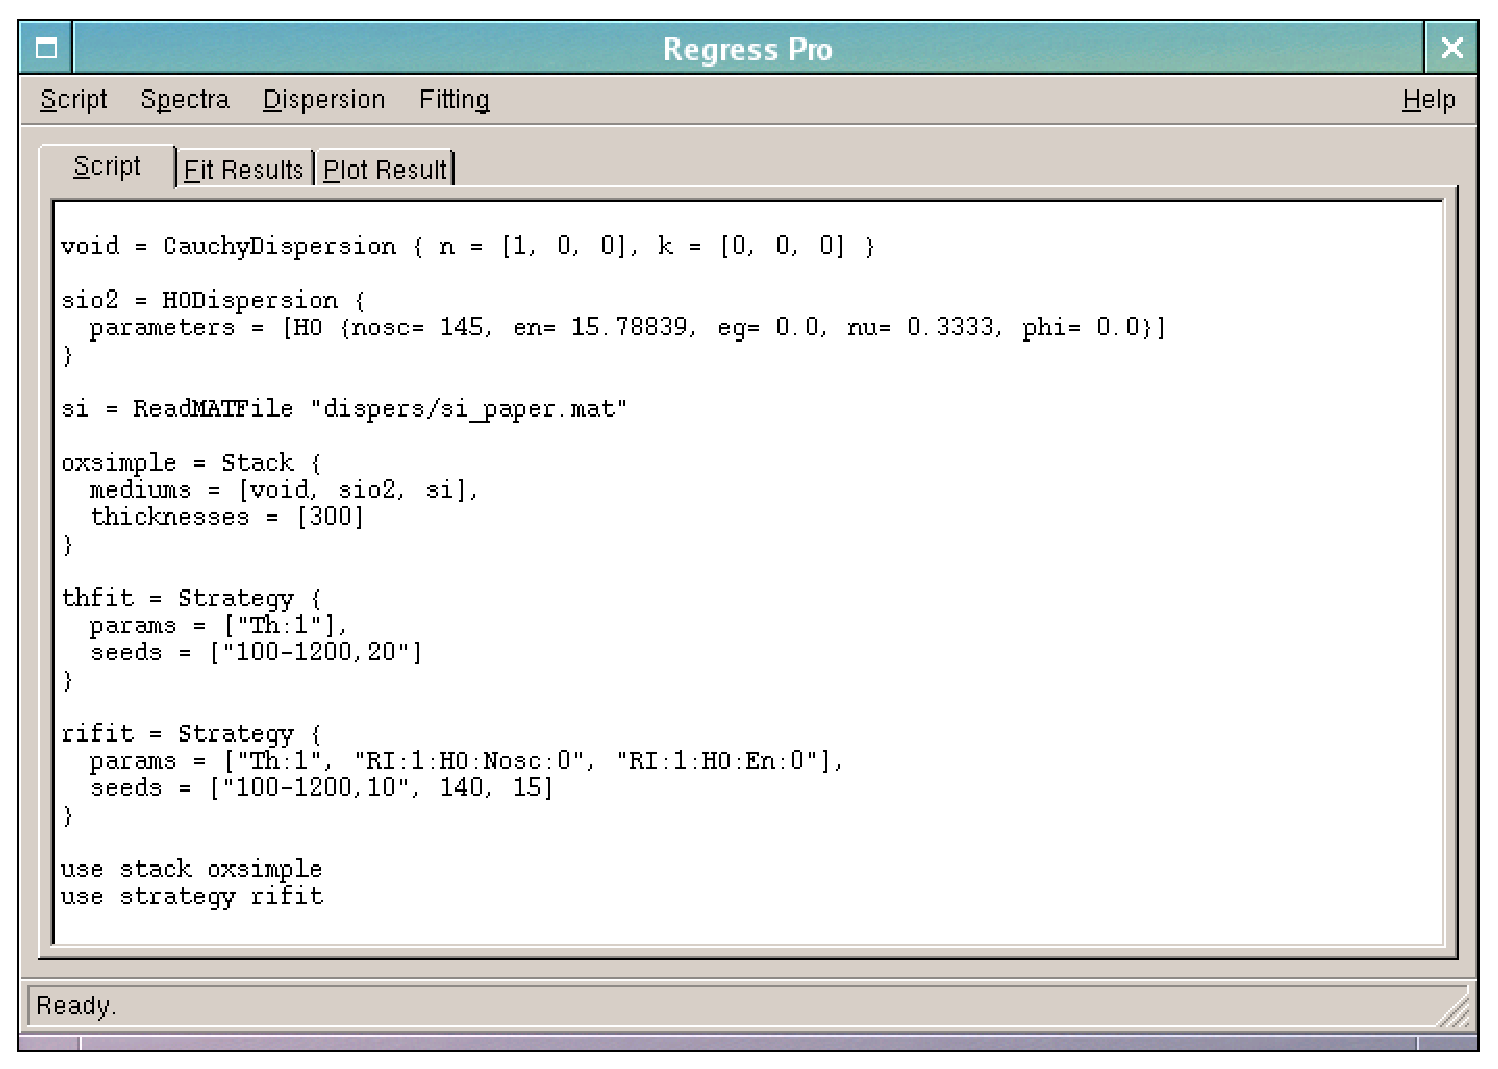
\includegraphics[width=\textwidth]{figure/script-window.eps}
  \caption{Script example with Regress Pro}
\end{figure}

\section{Film Stack description}
Before defining the film stack you have to define each of the involved
materials. Let's suppose that you want to define a simple oxide on
silicon film stack. Then you declare the material in the following way
\begin{verbatim}
void = CauchyDispersion { n = [1, 0, 0], k = [0, 0, 0] }

sio2 = ReadNKFile "dispers/thermal-sio2.nk"

si = ReadMATFile "dispers/si_paper.mat"
\end{verbatim}
In the first row we define the ``void'' material to describe the air
of the environment. Since we can approximate the air as having a
refractive index of 1 at all the wavelengths we can describe it with a
trivial Cauchy model, as indicated. Then, to describe the oxide we
have used the ``ReadNKFile'' function in order to load a dispersion
curve in nk format. The same thing has been done for the silicon with
the difference that in this case the table is in ``MAT''
format. Regress Pro is able to load both dispersion curve in nk format
and in MAT format.

In this case we can do something more interesting to describe the
oxide, we can describe it with an harmonic oscillators model. In this
case our definition will look like
\begin{verbatim}
sio2 = HODispersion {
  parameters = [HO {nosc= 145, en= 15.78839, eg= 0.0, nu= 0.3333,
                    phi= 0.0}]
}
\end{verbatim}
The definition is quite self-explanatory. We are using the
``HODispersion'' tag to define an Harmonic Oscillator model. Then in
the field ``parameters'' we define all the parameters of the harmonicl
oscillators. The use of the square backet '[' means that here we can
provide, potentially, a list of comma separated values. In particular,
in this case, we can write in the list one term for each of the
harmonic oscillator that we want to use in the model. In this case we
have just one harmonic oscillator. Then, for each oscillator, we
provide 5 parameters:
\begin{itemize}
  \item nosc, Number of Oscillators for $\textrm{cm}^3$
  \item en, The Energy of the Oscillator, expessed in eV
  \item eg, The Absorption Bandwidth of the oscillator, expressed in
  eV
  \item nu, the Local Field Effect coefficient, normally you can keep
  it to the value of 1/3
  \item phi, the Phase of the Oscillator term, useful to describe
  absorbing peak in the DUV region
\end{itemize}
In this case we can keep ``eg'' and ``phi'' at 0 since the silicon
oxide is a non-absorbing dielectric.

Once we have defined all the materials we can easily describe the film
stack as follows
\begin{verbatim}
oxsimple = Stack {
  mediums = [void, sio2, si],
  thicknesses = [300]
}
\end{verbatim}

Even in this case the definition is quite self-explanatory. We have
defined a film stack, that we call ``oxsimple'', by using the tag
``Stack''. Then we define
\begin{itemize}
  \item the list of the mediums (materials composing the film stack)
  \item the default thicknesses for each layer
\end{itemize}
The definition of the mediums begin from the top and it ends with the
substrate at the bottom. In this case we have the sequence void, sio2
and si. Note that all the materials referenced here has been defined
previously in the script. In the ``thicknesses'' we provide just one
value, which is the thickness of the oxide layer. Note that this is a
default value and it can be changed if we decide to fit this
parameters.

\section{Fit Strategy Definition}
The next step after the definition of the film stack is to define the
fit strategy. It will define which parameters will be fitted, the seed
values and, in case, an uniformily spaced grid to search the best fit
value for a given parameters. Before to explain in detail the fit
strategy concept lets continue the previous example by defining a fit
strategy. It we want to fit only the thickness of the oxide we can
define something like that
\begin{verbatim}
thfit = Strategy {
  params = ["Th:1"],
  seeds = ["100-1200,20"]
}
\end{verbatim}
You can note that the tag to define a strategy is ``Strategy''. In
this case we have called our strategy ``thfit''. In the field
``params'' we will give a list of all the parameter that we want to
fit. We will provide later a detailed specification to describe all
the possible fit parameters. In the mean time, let's say that ``Th:1''
is the thickness of the layer 1. In Regress Pro the layer are numbered
from the top to the bottom. The layer 1 being the top most film layer
of the stack. Then we have defined the ``seeds'' field. This latter
gives the seed value for each of the parameters defined in
``params''. A seeds can be of two different type
\begin{itemize}
  \item a simple seed, just a number to be used as seed value
  \item a range specification of the form ``a-b,delta'' where a, b and
  delta are, respectively, the minimum, the maximum and the stride of
  the search grid, expressed in nm
\end{itemize}
As a matter of fact, if there is at least one parameters which gives
the seed specification if the form of a range, then a grid search will
be effectuated before starting the actual fit. The grid search is
useful because the fit algorithm is able to converge only if the seed
value is near enough to the solution. This is especially true for fit
of ellipsometric data because the model is strongly not-linear in its
parameters.

Let us provide, for the given example, another possible strategy that
we can define. This latter will be a fit strategy to determine both
the thickness and the refractive index of the oxide. It will look like
\begin{verbatim}
  rifit = Strategy {
  params = ["Th:1", "RI:1:HO:Nosc:0", "RI:1:HO:En:0"],
  seeds = ["100-1200,10", 140, 15]
}
\end{verbatim}
You can note that we have used a different name for differetiate this
strategy from the strategy defined before. If you look at the list of
the fit parameters you will see that the fist one is always the
thickness and we have added to more fit parameters to vary the
``Nosc'' and ``En'' paramter of the oxide. Note that this will work
correctly only if the oxide was defined with an harmonic oscillators
model. We will give a detailed explanation about the format of the fit
parameters laters. You can note that, for the two latter fit
parameters, we have provide a simple seed, without any range
specification. This is fine since we expect that, for un oxide like
material, the actual values of these parameters will be not far from
those of a thermal oxide.

A script will always terminate with some ``use'' directives like these
\begin{verbatim}
  use stack oxsimple
  use strategy thfit
\end{verbatim}
The directives are needed to specify which stack and which fit
strategy should be used because several film stack and fit strategies
can be defined within a single script.

\subsection{Fit Parameter Format}
The fit parameters are specified with a string. It will be in the
format ``Th:n'', where ``n'' is an integer, to specify the thickness of
the layer n. If you want to specify a fit parameter for the dispersion
model of one of the fit layers you should use the format
``RI:n:MODEL'', where n is still the layer number and MODEL is a
string that depends from the model which is actually used for the
film. For example, if the model is an harmonic oscillator it can be
the string ``HO:Nosc:i'', where HO specify that we expect an harmonic
oscillator model, ``Nosc'' indicates the parameter ``number of
oscillators'' and ``i'' is an integer that individuate the oscillator,
since a model can employ several different oscillators.

\subsection{The Grid strategy}
The grid strategy can be used when a given parameter should be
determined over a big range of variation. In this case you cannot
limit yourself to provide a seed value because the fit will not
converge. Regress Pro allows to use ``grid search'' approach that will
permit to explor a big window of variation for some (or all) of the
fit parameters. The grid will be used automatically if you define at
least one parameter in the form ``min-max,delta''. Please be careful
when you specify a grid search over several parameters because,
depending on the stride of each parameter, the grid search can be very
time consuming.

The general concept of the grid search is the following. All the
points defined by the grid will be tested and the corresponding
$\chi^2$ is evaluated. If the $\chi^2$ is less then a given thresold
(determined with the \textbf{set chisq\_thresold} directive) the point
is considered a good starting point. Then the point is used as a seed
to start the real fit. If you do not specify the thresold value for
the $\chi^2$ a predefined value will be used depending on the nature
of the spectrum that is loaded.

\subsection{``Use'' Directives}
The use directives allows to configure some global parameters of the
fit like ``max\_iterations'', ``chisq\_thresold'', ``range'' and
``subsampling''. The parameter ``chisq\_thresold'', in particular, is
useful because it determines when a point evaluated during the grid
search should be considered good enough to start the actual fit.

\chapter{Running a Fit}
To actual running a fit you have to
\begin{enumerate}
  \item define or load a script
  \item load a spectrum.
\end{enumerate}
To load a spectrum you can use the function of the menu. The spectrum
should be in a format specific of Regress Pro. This format is in ASCII
format and is very easy to understand. You can just look to the
examples provided with Regress Pro to understand how the data should
be formatted.

Once you have loaded a spectrum you can start the fitting by using the
function of the menu ``\textsf{Fitting $\rightarrow$ Run Fitting}''. If the
fitting has been successful the results will be presented in the tabs
``Fit results'' and ``Plot results''. In ``Fit results'' you will find
the results of the fit plus some informations, more or less
useful. Then in the ``Plot results'' tab you will find a plot with the
experimental spectrum and the model. The golden rule of spectroscopic
ellipsometry is that \emph{a fit is good if the model corresponds to
the experimental spectrum}.

In the figure you will find un example of a successful fit.
\begin{figure}[!thp]
  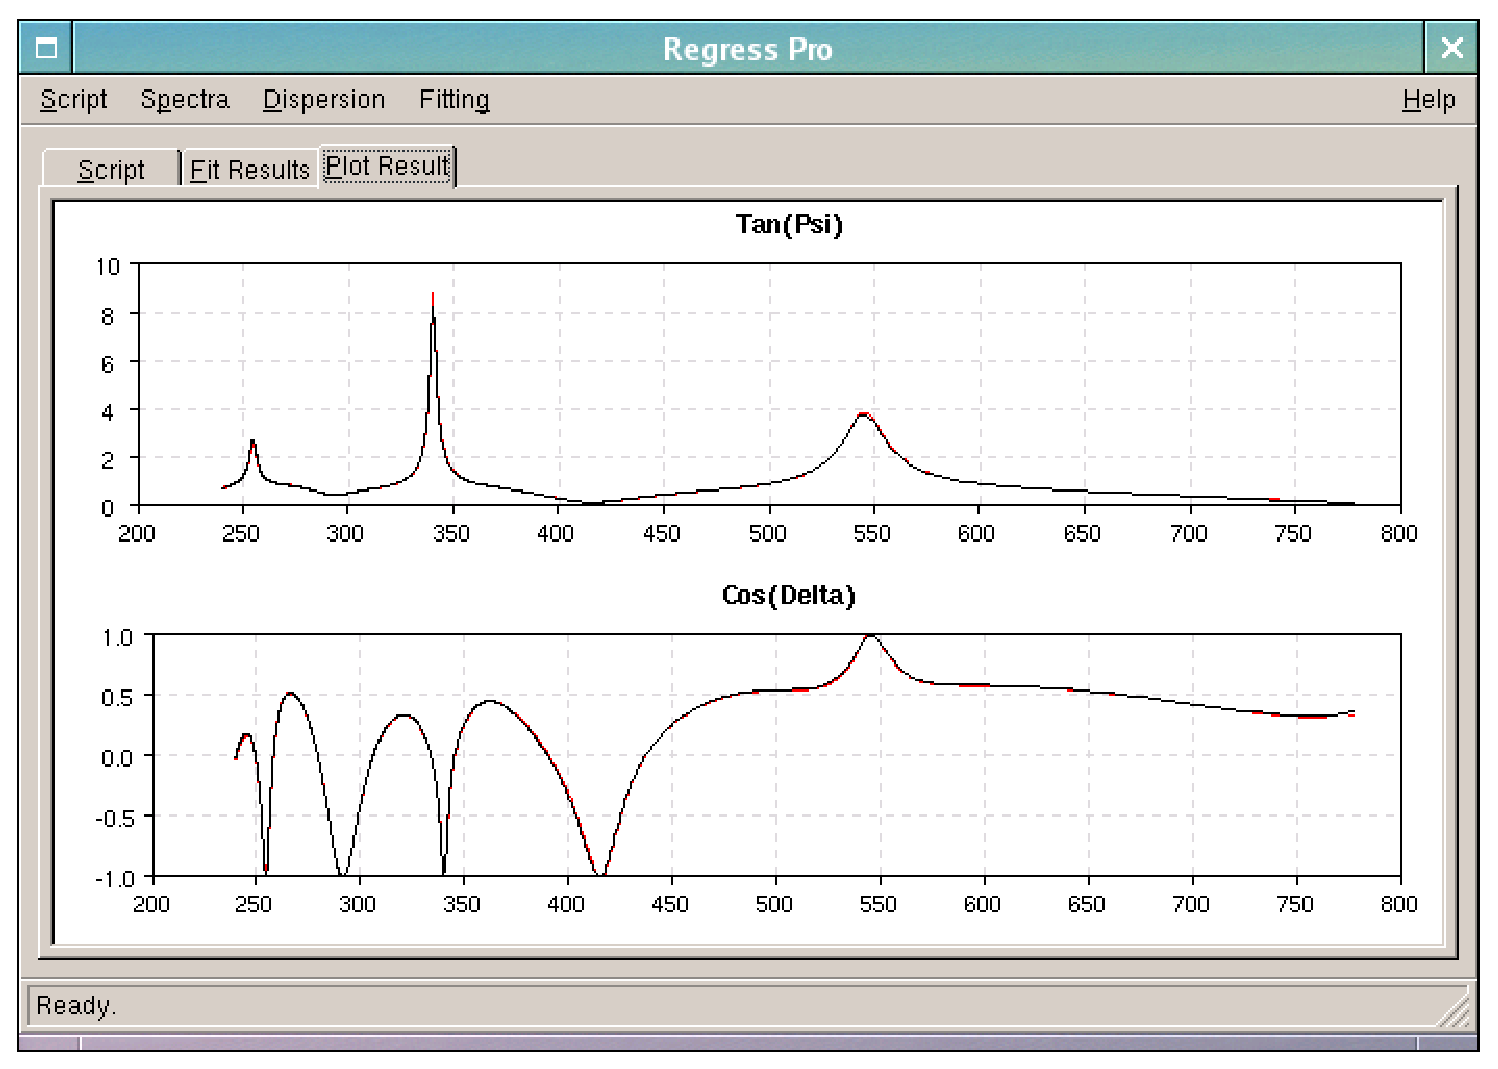
\includegraphics[width=\textwidth]{figure/oxide-fit-1.eps}
  \caption{Fit of a ellipsometric fit of a silicon oxide}
\end{figure}

\end{document}
